\documentclass[12pt, a4paper]{article}

\usepackage[utf8]{inputenc}
\usepackage[T1]{fontenc}
\usepackage[portuguese]{babel}
\usepackage{amsmath, amssymb, amsfonts}
\usepackage{graphicx}
\usepackage{geometry}
\usepackage{tikz}
\usepackage{xcolor}
\usepackage{float}
\usepackage{subcaption}
\usepackage{booktabs}

\geometry{top=2cm, bottom=3cm, left=3cm, right=2cm}

\title{(Universidade de São Paulo)\\
Resolução Numérica de uma Equação Elíptica via Método de Diferenças Finitas de Segunda Ordem}

\author{Métodos Numéricos em Equações Diferenciais\\
Docente: Fabrício Simeoni de Sousa\\[.2cm]
\begin{tabular}{r@{\ }c@{\ }l}
    Kainã Alves Tureso      &-- &15466391\\
    Vinícius de Sá Ferreira &-- &15491650
\end{tabular}}

\date{\today}

\begin{document}

    \maketitle

    \tableofcontents

    \vfill
    \begin{abstract}
        Este documento apresenta a formulação matemática e a discretização de um problema de valor de contorno bidimensional utilizando o Método de Diferenças Finitas (MDF). O modelo envolve uma Equação Diferencial Parcial (EDP) elíptica com condições de contorno mistas (Dirichlet, Neumann e Robin). O problema contínuo é transposto para o domínio discreto via aproximações de derivadas de ordem $\mathcal{O}(h^2)$, culminando na montagem de um sistema linear cujos coeficientes são organizados eficientemente através do produto de Kronecker. Por fim, realiza-se uma análise computacional dos resultados e da convergência numérica do método.
    \end{abstract}

    \section{Introdução e Formulação do Problema}

    O foco do presente estudo é a obtenção da solução numérica, denotada por $u(x,y)$, para a seguinte Equação Diferencial Parcial definida no domínio $\Omega = [0,1] \times [-1,1]$:
    \begin{equation}
        \frac{\partial^2 u}{\partial x^2}(x,y) + 3\frac{\partial^2 u}{\partial y^2}(x,y) = (4\pi^2-3)\frac{\partial u}{\partial y}(x,y), \quad (x,y) \in \Omega. \label{eq}
    \end{equation}

    As fronteiras do domínio estão sujeitas a diferentes condições. Nas extremidades laterais, impõe-se a condição de Dirichlet homogênea:
    \begin{equation}
        u(0,y) = u(1,y) = 0, \quad y \in [-1,1]. \label{dirichlet}
    \end{equation}

    Nas fronteiras inferior e superior, o problema é governado por condições envolvendo a derivada normal à superfície:
    \begin{equation}
        \frac{\partial u}{\partial \mathbf{n}}(x,-1) = e \sin(2\pi x),\quad \frac{\partial u }{\partial \mathbf{n}}(x,1) + u(x,1) = 0, \quad x \in [0,1]. \label{neumann}
    \end{equation}

    Para o desenvolvimento numérico, é conveniente explicitar as derivadas normais. Sendo o vetor normal às bordas verticais dado por $\mathbf{n}(x,y) = \begin{pmatrix}0 & y\end{pmatrix}^T$ para $(x,y)\! \in\! (0,1) \times \{-1,1\}$, a condição de Neumman na borda inferior ($y = -1$) traduz-se em:
    \[\begin{pmatrix}\frac{\partial u}{\partial x}(x,-1) & \frac{\partial u}{\partial y}(x,-1)\end{pmatrix} \begin{pmatrix}0 \\ -1\end{pmatrix} = e \sin(2\pi x) \iff -\frac{\partial u}{\partial y}(x,-1) = e \sin(2\pi x).\]

    De maneira análoga, para a borda superior ($y = 1$), a condição de Robin torna-se:
    \[\begin{pmatrix}\frac{\partial u}{\partial x}(x,1) & \frac{\partial u}{\partial y}(x,1)\end{pmatrix} \begin{pmatrix}0 \\ 1\end{pmatrix} + u(x,1) = 0 \iff \frac{\partial u}{\partial y}(x,1) + u(x,1) = 0.\]

    Deste modo, as condições de contorno de Neumann e Robin em \eqref{neumann} são reescritas como:
    \begin{equation}
        -\frac{\partial u}{\partial y}(x,-1) = e \sin(2\pi x),\quad \frac{\partial u}{\partial y}(x,1) + u(x,1) = 0, \quad x \in [0,1]. \label{neumann_remake}
    \end{equation}


    \section{Metodologia de Discretização Numérica}

    Para obter a solução do sistema \eqref{eq}-\eqref{neumann_remake}, emprega-se o método de diferenças finitas com aproximações centradas para a primeira e segunda derivadas, assegurando precisão espacial de ordem $\mathcal{O}(h^2)$:
    \[u'(x_n) \approx Du(x_n) = \frac{u(x_{n+1})-u(x_{n-1})}{2h}\]
    \[u''(x_n) \approx D^2u(x_n) = \frac{u(x_{n-1})-2u(x_n)+u(x_{n+1})}{h^2}\]

    Estabelece-se uma malha uniforme com espaçamento $h = \frac{1}{n+1} = \frac{2}{m+1}$. Os nós da malha são definidos pelas coordenadas $x_i = ih$ e $y_j = -1 + jh$, para os índices $i \in \{0,1,\cdots,n+1\}$ e $j \in \{0,1,\cdots,m+1\}$. Denotando a aproximação numérica por $U_{i,j} \approx u(x_i, y_j)$, a versão discreta da equação \eqref{eq} para os pontos interiores passa a ser:
    \begin{equation}
        \frac{U_{i-1,j}-2U_{i,j}+U_{i+1,j}}{h^2} + 3\left(\frac{U_{i,j-1}-2U_{i,j}+U_{i,j+1}}{h^2}\right) = (4\pi^2-3)\frac{U_{i,j+1}-U_{i,j-1}}{2h}. \label{num_eq}
    \end{equation}

    As condições de fronteira, correspondentes às Equações \eqref{dirichlet} e \eqref{neumann_remake}, tomam a forma:
    \begin{align}
        &{\color{red}U_{0,j}} = {\color{red}U_{n+1,j}} = 0, \quad j \in \{0,\cdots,m+1\} \label{num_dirichlet}\\
        &-\left(\frac{U_{i,1}-U_{i,-1}}{2h}\right) = e \sin(2\pi x_i),\quad \frac{U_{i,m+2}-U_{i,m}}{2h} + U_{i,m+1} = 0, \quad i \in \{1,\cdots,n\}. \label{num_neumann}
    \end{align}

    Para preservar a ordem $\mathcal{O}(h^2)$ do esquema nas fronteiras horizontais \eqref{num_neumann}, introduzimos camadas de pontos fantasmas (nós fictícios) externos ao domínio, denotados por $U_{i,-1}$ e $U_{i,m+2}$. Isolando estes termos, obtemos suas expressões em função dos pontos reais da malha:
    \begin{equation}
        U_{i, -1} = U_{i, 1} + 2he\sin(2\pi ih),\quad U_{i,m+2} = U_{i,m} - 2h U_{i,m+1}. \label{simp_neumann}
    \end{equation}

    Substituindo estas relações no estêncil dos pontos pertencentes à fronteira física, as equações governantes do problema podem ser simplificadas e consolidadas na seguinte estrutura para todos os pontos a serem calculados:
    \begin{equation}
        \frac{1}{h^2}(U_{i-1,j} + U_{i+1,j} - 8 U_{i,j}) + \left(\frac{3}{h^2} + \frac{4\pi^2 -3}{2h}\right)U_{i,j-1} + \left(\frac{3}{h^2} - \frac{4\pi^2 -3}{2h}\right) U_{i,j+1} = 0 \label{simp_eq}
    \end{equation}
    com as devidas substituições sendo ativadas nos contornos.


    \section{Modelagem Algébrica e Construção do Sistema Linear}

    Para a resolução computacional, as incógnitas $U_{i,j}$ localizadas no interior e nas fronteiras com condições derivadas devem ser mapeadas para um vetor unidimensional $\mathbf{U}$. Utiliza-se um ordenamento lexicográfico (varrendo $i$ de $1$ a $n$, e depois $j$ de $0$ a $m+1$), sendo:
    \[\mathbf{U} = \begin{pmatrix}
        \color{blue}U_1\\
        \color{blue}U_2\\
        \vdots\\
        \color{blue}U_n\\
        U_{n+1}\\
        \vdots\\
        \color{blue}U_{n(m+2)}
    \end{pmatrix} \quad \text{onde} \quad U_k = U_{i,j},\ k = i + nj.\]

    A disposição espacial dos nós, distinguindo os pontos de Dirichlet (vermelhos) dos pontos a serem computados (azuis e pretos), pode ser observada no esquema geométrico abaixo:
    \begin{figure}[H]
        \centering
        \begin{tikzpicture}[scale=0.85, x=1cm, y=1cm]
            % linhas verticais
            \draw (1,0) -- (1,1); \draw (1,2) -- (1,4);
            \draw (2,0) -- (2,1); \draw (2,2) -- (2,4);
            \draw (3,0) -- (3,1); \draw (3,2) -- (3,4);
            \draw (4,0) -- (4,1); \draw (4,2) -- (4,4);

            % linhas horizontais
            \draw (0,1) -- (1,1); \draw (2,1) -- (4,1);
            \draw (0,2) -- (1,2); \draw (2,2) -- (4,2);
            \draw (0,3) -- (1,3); \draw (2,3) -- (4,3);
            \draw (0,4) -- (1,4); \draw (2,4) -- (4,4);

            % reticências horizontais
            \node at (1.55,0) {$\cdots$};
            \node at (1.55,1) {$\cdots$};
            \node at (1.55,2) {$\cdots$};
            \node at (1.55,3) {$\cdots$};
            \node at (1.55,4) {$\cdots$};

            % reticências verticais
            \node at (0,1.6) {$\vdots$};
            \node at (1,1.6) {$\vdots$};
            \node at (2,1.6) {$\vdots$};
            \node at (3,1.6) {$\vdots$};
            \node at (4,1.6) {$\vdots$};

            % reticências diagonais
            \node at (1.5,1.6) {$\ddots$};

            % eixos
            \draw[-] (-0.5,0) -- (1,0);
            \draw[->] (2,0) -- (4+0.5,0) node[right] {$i$};
            \draw[-] (0,-0.5) -- (0,1);
            \draw[->] (0,2) -- (0,4+0.5) node[above] {$j$};

            % pontos visíveis
            \foreach \i in {1,2,3}
            \foreach \j in {0,4}
                \fill[blue] (\i,\j) circle (2pt);

            \foreach \i in {0,4}
            \foreach \j in {0,1,2,3,4}
                \fill[red] (\i,\j) circle (2pt);

            \foreach \i in {1,2,3}
            \foreach \j in {1,2,3}
                \fill (\i,\j) circle (2pt);

            % rótulos simbólicos
            \node at (4,-0.4) {$n+1$};
            \node at (-0.9,4) {$m+1$};
            \node[below left] at (0,0) {$0$};
        \end{tikzpicture}
        \caption{Malha computacional ilustrando pontos de contorno e domínio interno.}
    \end{figure}

    A aplicação das equações \eqref{simp_eq} com a substituição das aproximações por nós fantasmas nas fronteiras horizontais \eqref{simp_neumann} leva a modificações no estêncil para $j=0$ e $j=m+1$. Com a notação linearizada $U_k$ (e definindo $U_0 = U_{n(m+2)+1} = 0$ devido ao contorno lateral), formamos o sistema linear unificado, para $i \in \{1,\cdots,n\}$ e, respectivamente, para $j=0$, $j \in \{1,\cdots,m\}$ e $j=m+1$:
    \begin{equation}
    \begin{cases}
        \displaystyle \frac{1}{h^2}(U_{i-1} + U_{i+1} - 8 U_{i}) + \frac{6}{h^2} U_{i+n} = -\left(\frac{6}{h} + 4\pi^2 -3\right)e\sin(2\pi ih)\\[.5cm]
        \resizebox{0.95\textwidth}{!}{$\displaystyle \frac{1}{h^2}(U_{i-1+nj} + U_{i+1+nj} - 8 U_{i+nj}) + \left(\frac{3}{h^2} + \frac{4\pi^2 -3}{2h}\right)U_{i+n(j-1)} + \left(\frac{3}{h^2} - \frac{4\pi^2 -3}{2h}\right) U_{i+n(j+1)} = 0$}\\[.5cm]
        \displaystyle \frac{1}{h^2}(U_{i-1+n(m+1)} + U_{i+1+n(m+1)}) + \left(4\pi^2 -3 -\frac{8}{h^2} - \frac{6}{h}\right)U_{i+n(m+1)} + \frac{6}{h^2} U_{i+nm} = 0
    \end{cases}
    \end{equation}

    \subsection{Representação Matricial do Sistema}

    Para o sistema $M \mathbf{U} = \mathbf{F}$, definimos as grandezas:
    \[\alpha(h) = \frac{3}{h^2}+\frac{4\pi^2 - 3}{2h},\quad \beta(h) = \frac{3}{h^2}-\frac{4\pi^2 - 3}{2h}.\]

    Utilizando a propriedade do produto de Kronecker, a matriz de coeficientes $M$, de dimensões $n(m+2) \times n(m+2)$, é montada da forma:
    \[M = (I_{m+2} \otimes T_{n} + T_{m+2} \otimes I_{n}) + (P_{-n}+Q_{+n}) + G_0\]
    Onde $I_k$ são matrizes identidade, e os blocos tridiagonais característicos dos esquemas de diferença central em cada direção são dados por:
    \[T_n = \begin{pmatrix}
        -\frac{4}{h^2} & \frac{1}{h^2} & 0 & \cdots & 0 \\
        \frac{1}{h^2} & -\frac{4}{h^2} & \frac{1}{h^2} & \cdots & 0 \\
        0 & \frac{1}{h^2} & -\frac{4}{h^2} & \ddots & \vdots \\
        \vdots & \ddots & \ddots & \ddots & \frac{1}{h^2} \\
        0 & \cdots & 0 & \frac{1}{h^2} & -\frac{4}{h^2}
    \end{pmatrix}_{n \times n}\!\!\!\!\!\!\!\!\!\!,\!\!\!\!\! \quad T_{m+2} = \begin{pmatrix}
        -\frac{4}{h^2} & \beta(h) & 0 & \cdots & 0 \\
        \alpha(h) & -\frac{4}{h^2} & \beta(h) & \cdots & 0 \\
        0 & \alpha(h) & -\frac{4}{h^2} & \ddots & \vdots \\
        \vdots & \ddots & \ddots & \ddots & \beta(h) \\
        0 & \cdots & 0 & \alpha(h) & -\frac{4}{h^2}
    \end{pmatrix}_{(m+2) \times (m+2)}\]

    Os termos $P_{-n}$, $Q_{+n}$ e $G_0$ atuam como correções esparsas nas posições referentes aos contornos verticais modificados pelas Equações de Neumann e Robin:
    \[(P_{-n})_{i,j} = \begin{cases}
        \displaystyle \beta(h), \text{ se $j = i-n$ e $i > n(m+1)$}\\[.2cm]
        0, \text{ caso contrário}
    \end{cases}\!\!\!\!\!\!,\, (Q_{+n})_{i,j} = \begin{cases}
        \displaystyle \alpha(h), \text{ se $j = i+n$ e $i \leq n$}\\[.2cm]
        0, \text{ caso contrário}
    \end{cases}\]
    \[(G_0)_{i,j} = \begin{cases}
        \displaystyle -2h\beta(h), \text{ se $i > n(m+1)$}\\[.2cm]
        0, \text{ caso contrário}
    \end{cases}\]
    
    O vetor de termos independentes carrega os estímulos das fronteiras:
    \[(F)_{i} = \begin{cases}
        \displaystyle -2h\alpha(h)e\sin(2\pi ih), & \text{se } i \leq n\\[.2cm]
        0, & \text{caso contrário}.
    \end{cases}\]

    \section{Resultados e Discussões}

    Utilizando \texttt{Python} e a biblioteca \texttt{NumPy}, o sistema matricial desenvolvido foi resolvido computacionalmente para a obtenção das distribuições térmicas no domínio. Os resultados apresentados a seguir foram gerados com um espaçamento de malha $h=0.010 \leq 0.1$, o que permite uma visualização precisa do comportamento da solução em comparação ao modelo analítico.

    \subsection{Comparação Analítica e Numérica}

    A primeira etapa da validação consiste na análise qualitativa da superfície numérica, obtida pela resolução de $M \mathbf{U} = \mathbf{F}$, em relação à superfície da solução analítica (referência) gerada nos exatos pontos da malha estipulada.

    \begin{figure}[H]
        \centering
        \begin{subfigure}{0.48\textwidth}
            \centering
            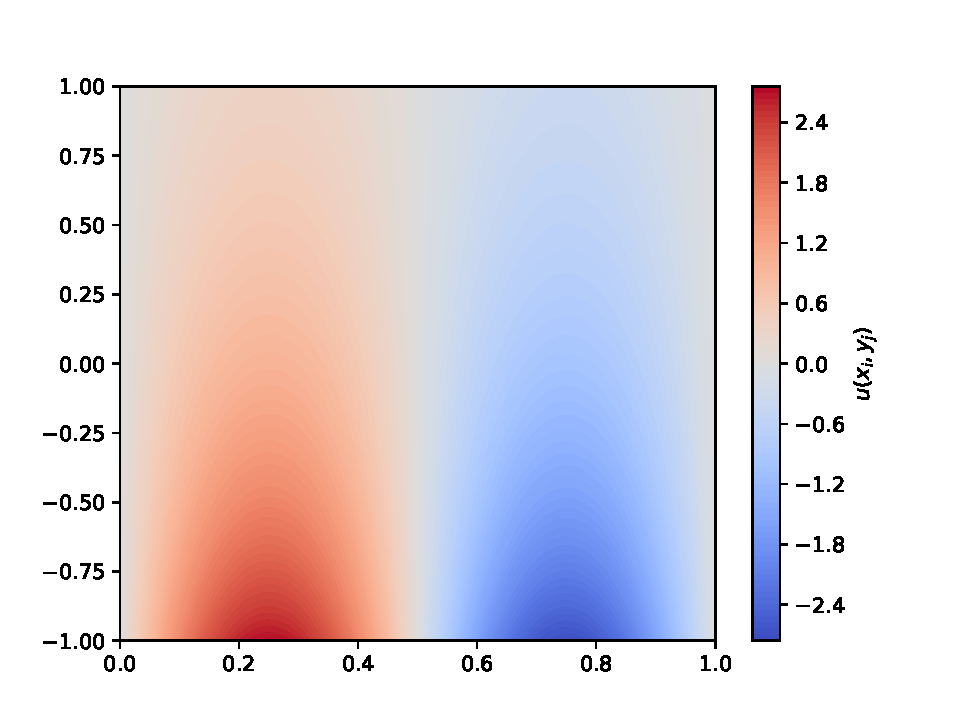
\includegraphics[width=\linewidth]{../images/analitico2D/h=0.010.pdf}
            \caption{Solução Analítica (Referência)}
        \end{subfigure}\hfill
        \begin{subfigure}{0.48\textwidth}
            \centering
            
\includegraphics[width=\linewidth]{../images/calculado2D/h=0.010.pdf}
            \caption{Solução Numérica ($h=0.010$)}
        \end{subfigure}
        \caption{Curvas de nível das soluções avaliadas no domínio para uma malha uniforme.}
        \label{fig:curvas}
    \end{figure}

    \begin{figure}[H]
        \centering
        \begin{subfigure}{0.48\textwidth}
            \centering
            
\includegraphics[width=\linewidth]{../images/analitico3D/h=0.010.pdf}
            \caption{Solução Analítica (Referência)}
        \end{subfigure}\hfill
        \begin{subfigure}{0.48\textwidth}
            \centering
            
\includegraphics[width=\linewidth]{../images/calculado3D/h=0.010.pdf}
            \caption{Solução Numérica ($h=0.010$)}
        \end{subfigure}
        \caption{Superfícies 3D das soluções avaliadas no domínio para uma malha uniforme.}
        \label{fig:superficies}
    \end{figure}

    Observando a Figura \ref{fig:superficies}, a concordância macroscópica visual entre as duas superfícies é uma forte evidência da corretude da modelagem do sistema, incluindo os coeficientes, as substituições das equações normais e as imposições de Dirichlet. 

    \subsection{Análise do Erro Absoluto Espacial}

    Defina o erro absoluto $e_{i,j} = |U_{i,j} - u(x_i, y_j)|$, em que $u$ é a solução analítica. Para comprovar essa similaridade, observamos as seguintes métricas sobre $e_{i,j}$: norma infinito, norma-1 e erro ponto a ponto. 
    \begin{table}[H]
        \centering
        \begin{tabular}{c|c|c}
            h       & $||e_{i,j}||_\infty$  & $||e_{i,j}||_1$ \\
            \hline
            $1/10$  & 0.0802                & 0.0815\\
            $1/25$  & 0.0133                & 0.0128\\
            $1/50$  & 0.0033                & 0.0032\\
            $1/75$  & 0.0015                & 0.0014\\
            $1/100$ & 0.0008                & 0.0008\\
        \end{tabular}
        \caption{Norma do erro}
        \label{table:erros}
    \end{table}

    Na tabela \ref{table:erros} é possível ver que as duas normas do erro diminuem conforme $h$ decresce. A análise do erro com $||\cdot||_\infty$ nos dá uma forte indicação de convergência, pois ela nos diz que em todo ponto em que está sendo feita a aproximação, o erro decresce.
    
    Para quantificar a dispersão do erro no domínio, calculou-se a diferença absoluta ponto a ponto entre a matriz analítica e a numérica. O comportamento dessa difração está ilustrado na Figura \ref{fig:erro_absoluto}.
    \begin{figure}[H]
        \centering
        
\includegraphics[width=0.6\linewidth]{../images/dif/h=0.010.pdf}
        \caption{Erro absoluto ponto a ponto ($h=0.010$)}
        \label{fig:erro_absoluto}
    \end{figure}
    
    Para além disso, a figura \ref{fig:erro_absoluto} nos mostra que os erros se concentram nas duas partes que apresentam curvatura mais acentuada. Este fenômeno decorre da natureza da condição de Neumann imposta ($e\sin(2\pi x)$); o erro de truncamento das diferenças finitas centrais é proporcional às derivadas de ordem superior da solução. Portanto, nos picos de amplitude da função seno (em $x = 1/4$ e $x = 3/4$), onde a norma da curvatura e do gradiente da solução são máximos, a aproximação por pontos fantasmas introduz as maiores discrepâncias. À medida que $y$ aumenta, observa-se uma dissipação desses resíduos, característica de problemas elípticos onde a influência das incertezas de contorno é atenuada pela suavização intrínseca do operador diferencial no interior do domínio.

    \subsection{Estudo de Convergência}

    Para atestar o rigor do esquema concebido, realizou-se o estudo do erro em malhas progressivamente refinadas: $h = \{1/10,\, 1/25,\, 1/50,\, 1/75,\, 1/100\}$. Avaliou-se o erro na norma infinito associado a cada espaçamento.

    \begin{figure}[H]
        \centering
        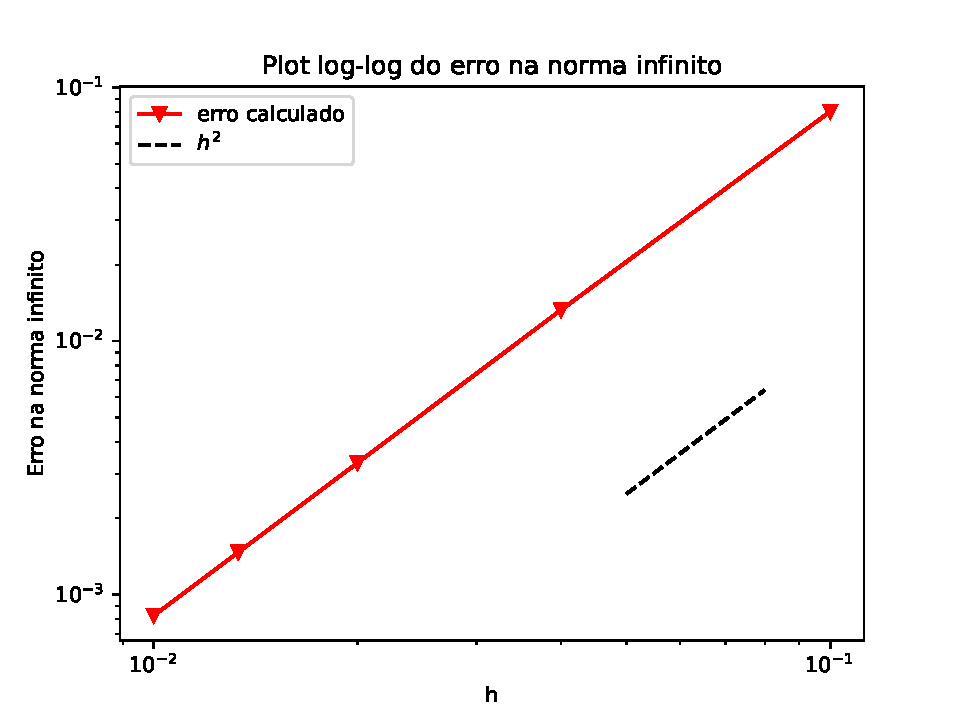
\includegraphics[width=0.6\linewidth]{../images/plot_loglog_erro.pdf}
        \caption{Curva de convergência numérica em escala logarítmica.}
        \label{fig:convergencia}
    \end{figure}

    O comportamento assintótico apresentado na Figura \ref{fig:convergencia} ratifica a validade da discretização de segunda ordem utilizada neste projeto. A inclinação da reta decrescente no gráfico log-log sinaliza a razão pela qual o erro decai à medida que $\log(h)$ diminui. Como esperado pela modelagem teórica proposta na Seção 2, verificamos que o erro global decai de modo compatível com a ordem quadrática $\mathcal{O}(h^2)$, comprovando que as simplificações e o tratamento de contorno via produto de Kronecker não prejudicaram a consistência da resposta numérica aproximada.

    \section{Conclusão}

    A conversão matricial de um problema de contorno envolvendo EDPs com diferentes restrições nas bordas demanda estruturação cuidadosa para não depreciar a ordem de precisão adotada no núcleo da malha. Através da criação dos operadores lineares via produto de Kronecker e da integração da condição fantasma dentro das faixas marginais ($T_n$ e $T_{m+2}$), o modelo implementado alcançou estabilidade notória. O estudo de caso com um $h \leq 0.1$ permitiu averiguar que o erro do sistema converge eficientemente a zero com a redução espacial simulada.

\end{document}